\documentclass[usegeometry=true]{scrartcl}
\usepackage[ngerman]{babel}
\usepackage[T1]{fontenc}
\usepackage{lmodern}
\usepackage[utf8]{inputenc}
\usepackage{hyperref}
\usepackage{amssymb}
\usepackage{graphicx}
% Dimensionen bitte nicht ändern. 
\usepackage[left=2cm, right=2cm, top=2cm, bottom=2cm, bindingoffset=1cm, includeheadfoot]{geometry}
%Zeilenabstand bitte nicht ändern
\usepackage[onehalfspacing]{setspace}


\bibliographystyle{unsrt}

\begin{document}
% ----------------------------------------------------------------------------
\subject{Projektbericht zum Modul Information Retrieval und Visualisierung Sommersemester 2021}

\title{Bike Buyers 1000}
%\subtitle{Untertitel}% optional
\author{Floyd Spuhler}% obligatorisch
\date{10.09.2021}
\maketitle% verwendet die zuvor gemachte Angaben zur Gestaltung eines Titels
% ----------------------------------------------------------------------------
% Inhaltsverzeichnis:
\newpage
\tableofcontents
% ----------------------------------------------------------------------------
% Gliederung und Text:
\newpage
\section{Einleitung}
Durch das wachsende Umweltbewusstsein in der Bevölkerung rückt besonders das Fahrrad als klimaneutrales Verkehrsmittel in den Fokus \cite{Marquart.2021}. Bereits 2019 betrug der Gesamtbestand an Fahrrädern in Deutschland fast 76 Millionen \cite{Kords.26.06.2020,Statista.25.08.2021}. Die anhaltende Covid-19 Krise verstärkt den anhaltenden Fahrrad-Boom für Freizeit und  Pendeln \cite{Platter.2020}. Durch die Krise bedingte Lieferverzögerungen und Knappheiten führen zu einem Nachfrageüberhang und steigenden Preisen. Auch wärmere Winter begünstigen eine längere Fahrradsaison und sorgen dadurch zusätzlich für Lieferengpässe \cite{tagesschau.11.03.2021}. Neuentwicklungen wie E-Bikes werden immer beliebter, was sich an der Gesamtabsatzbeteiligung im Jahr 2020 von 38,7\% bermerkbar macht \cite{tagesschau.11.03.2021}. 
In der Schweiz ist das Fahrrad nicht zuletzt durch den staatlich geförderten Ausbau von Fahrradspuren zum beliebtesten Verkehrsmittel geworden \cite{Platter.2020}.
\newline Fragestellungen: Welche Eigenschaften lassen sich aus den Bike-Buyers-Daten ableiten? Darstellungen: Scatterplot, Parallele Koordinaten

\subsection{Anwendungshintergrund}


Diese Forschungsarbeit bereitet Informationen auf, die Interessante Einblicke in das Kaufverhalten von Fahrrad-Kunden geben. So lassen sich anhand von Einkommensdaten, dem Alter und dem Bildungshintergrund Kundengruppen ableiten, auf welche in allen Wertschöpfungsebenen eingegangen werden kann. Hersteller müssen beispielsweise die Rahmengröße auf das Alter abstimmen. Einkommensstarke Kunden setzten den Fokus beispielsweise auf hochwertige Materialien (z.B. Carbon). Personen die das Fahrrad zum Pendeln nutzen sind eher auf ein Stadt- als ein Mountainbike angewiesen. Anhand der Distanz zur Arbeit können Bauunternehmen in Innenstädten gezielter Fahrradwege bauen. Diese Anwendungsfelder werden über die drei verschiedenen Visualisierungsanwendungen aufgegriffen. 

Mit einem Scatterplot, bestehend aus X und Y Achse, können Zusammenhänge von Y in Abhängigkeit von X festgestellt werden. Diese Zusammenhänge werden in Form von Punkten, die zwischen beiden Achsen liegen und einen Achsenwert darstellen, visualisiert. Dabei fallen die Beziehungen zwischen den beiden Punkten je nach  Verwendungszweck unterschiedlich stark aus \cite{Yi.16.10.2019,Anscombe.1973,Cleveland.1984}. Der Scatterplot wird für die Daten zu Fahrradkunden als erste Darstellung von Zusammenhängen verwendet. 

Mit der zweiten Visualisierung, Parallelen Koordinaten, können Zusammenhänge  multi-dimensionaler Daten besser als über Punkte dargestellt werden. Punkte werden dabei zu Achsenbeschriftungen und Linien \cite{Inselberg.1990}. (Inselberg)
Jede betrachtete Variable wird nebeneinander angeordnet. Alle dazugehörigen Datenwerte werden über eine Linie minenander verbunden \cite{Moustafa.2006}. 

Die vertikalen Achsen sind über Linienn miteinander verbunden. Die Auf- und Abbewegungen der Linien zeigen Werteveränderungen auf \cite{Few.2008}. 
Dabei sind die Achsen parallel zueinader angeordnet. Parallele Koordinaten bieten einen giten Datenüberblick. Eine Gefahr stellt allerdings die Überlappung von Linen dar, wenn zu viele Daten verwendet werden \cite{Heinrich.2009}.

Über die Buamhierarchie lassen sich Daten und deren Beziehungen untereinander anordnen, wodurch eine übersichtliche Datenstruktur entsteht und sich Daten schnell wiederfinden lassen. Die Baumstruktur besteht aus Knoten und Kanten. Zwei Knoten sind jeweils über eine Kante miteinander verbunden. In der Baumstruktur muss ein Knoten vorhanden sein, der keinen Vorgänger hat. DIeser Knoiten wird Wurzel genannt. Dessen Folgeknoten werden Nachfolger genannt. Über die Wurzel führen nur azyklische Pdade und zu jedem Knoten nur ein Pfad.  Durch die unterschiedlichen Pfade und Verzweigungen der unterschiedlichen Daten entsteht die Baumstruktur \cite{Gumm.2016}. (S. 289) Diese Visualisierungstechnik eignet sich für die übersichtliche Darstellung bestimmter Daten aus den BikeBuyern, da diese Daten Strukturen aufweisen, die sich als Hierarchien darstellen lassen.
Der hintergrund für die Auswahl dieser Form ist, dass sich die DAten in DFahrradkäufer und nicht-Käufergruppen unterteilen lassen. Des Weiteren sollen globale Unterschiede dargestellt werden, um auf territoriale Umfelder eingehen zu können. EIn weiter Faktoir ist die Pendlerdistanz vom Wohnsiotz der Befragten zur Arbeit, welche verschiedene Antwortmöglichkeiten zulässt. All diese Faktoren können Kombiniert in die Baumhierarchie übertragen werden.   
\subsection{Zielgruppen}
Dieser Forschungsbericht richtet sich vor allem an die Anbieterseite auf den B2C Fahrradmarkt. Auf der Anbieterseite sind alle in der Lieferkette vorhandenen Unternehmensbrachen betroffen. Die Hersteller haben mit dem Materialmangel zu kämpfen.Den Fahrradverkäufern macht der Onlinehandel Konkurrenz und auch Bauunternehmen, die Fahrradspuren bauen haben mit Rohstoffmangel Probleme.  Hierzu lassen sich drei Hauptzielgruppen, neben Fahrradinteressierten, herausfiltern, an welche sich dieser Visualisierungsbericht richtet.
\begin{itemize}
 \item \textbf{Fahrradhersteller}: 
 \newline Fahrradhersteller benötigen besonders wegen der Materialknappheit spezifische Informationen zu den personenbezogenen Merkmalen potenzieller Kunden, wie z.B. Größe, Alter, Einkommen um einen Fahrradrahmen mit entsprechend wertigen / nicht wertigen Materialien für eine Verwendungszweck (z.B. Mountainbike, Stadtrad)herzustellen 
 Für Fahrradhersteller sind Informationen zum Alter der Kundengruppe für Rahmengröße, Fahrradart, sowie zum Einkommen in Hinblick auf die Auswahl der Materialien und deren Qualität wichtig. 
 \item \textbf{Fahrradhandel}:
 \newline Für Fahrradverkäufer spielt vor allem der Verwendungszweck des potenziellen Kunden eine übergeordnete Rolle beim Fahrradkauf. Die Wahl des richtigen Modells unterscheidet sich für die Freizeit (Mountainbike) mit weiten Distanzen vom Gebrauch für die Stadt mit geringeren Distanzen (Stadtrad). Für weitere Distanzen eignen sich Mountainbikes besser als für die Fahrt in ebenerdigem Terrain, wie asphaltierten Straßen. für Stadträder. 

 \item \textbf{Bauunternehmen mit dem Fokus auf Fahrradinfrastruktur}:
 \newline Auch für Unternehmen aus der Baubranche mit dem Fokus auf die Infrastruktur für Fahrradwege ist diese Arbeit eine geeignete Anlaufstelle für Informationen zum Einsatz des Fahrrads in Bezug auf den Arbeitsweg. Daten zu Pendlerwegen müssen für diese Zielgruppe besonders aufgegliedert vorliegen, da Bauunternehmen somit Informationen über die benötigten Distanzen neuer Fahrradwege erhalten und besonders in Städten nur begrenzt Raum zur Verfügung haben. Dadurch muss der EInsatz von Baumaschinen beonsders abgewogen werden. 
 
\end{itemize}

Dieser Visualisierungsbericht ermöglicht es den oben genannten Unternehmen eine bessere Kundenmarktsegmentierung zu betreiben. Kurzfristig können durch die Ergebnisse dieses Berichtes Ressourcen sparsam eingesetzt werden (v.a. Hersteller, Baubranche). Langfristig können besonders Fahradhändler von diesem Bericht profitieren, da sie durch die personenbezogenen Daten optimale Kundenakquise / Kundenberatung garantieren können und anhand von Einkommensparametern Preise bestmöglich bilden können. 



\subsection{Überblick und Beiträge}
Die durch Kaggle bereitgestellten Daten bestehen aus demographischen Kundeninformationen, wie Alter, Geschlecht, Familienstand etc.  Diese Daten werden über die drei Visualisierungstechniken Scatterplot, Parallele Koordinaten und Baumhierarchie abgebildet, um den in 1.2 angesprochenen Zielgruppen einen Überblick in diese Kundendaten zu vermitteln.Über den Scatterplot können jeweils zwei Dateneigenschaften einander gegenübergestellt werden. Bei der Anwendung kann über Buttons selbst ausgewählt werden, welche beiden Eigenschaften angezeigt werden sollen. Mit den parallelen Koordinaten haben Interessenten die Möglichkeit über vertikale Achsen Werte miteinander zu vergleichen. Buttons ermöglichen hierbei die dynamische Achsenverschiebung. Die Baumhierarchie lässt die Daten anhand wesentlicher Eigenschaften in verschiedenen Ebenen darstellen. 

\section{Daten}
Die diesem Projektbericht zugrundeliegenden Rohdaten entstammen einem Datensatz des " Kaggle" -Account von Heeral Dedhia \cite{Dedhia.22.09.2020}, welche Antworten von 1.000 NutzerInnen zum Thema Fahrradkauf bereitstellt. Die Nutzerin hat diese Daten zuletzt im Jahresverlauf 2020 erweitert. Datum- und Erhebungsform sind hierbei unbekannt. In dieser aktuellsten Version liegen 13 verschiedene Attribute zu den 1000 befragten Personen vor. Die Nutzerin hat zwei verschiedene Datensätze bereitgestellt, die sich lediglich durch NA-Werte unterscheiden. Um bei einer Datenvorverarbeitung keine Daten zu vergessen und die Funktionsfähigkeit des Elm CSV-Decoders zu gewährleisten, stellt die bereinigte Datei "bikebuyersclean.csv" die Grundlage für dieses Visualisierungsprojekt dar (ToDo: Kaggle Seite zitieren). 

zu allen befragten personen wurde eine eindeugige ID vergeben, welche ein INT-Typ ist. Zur quantifizierung der Baumhierarchie wurde diese Tabellenspalte für die dritte Visualiserung übernommen. Die nächsten beiden Spalten "Marital Status" , "Gender" und "Children" und "Age" als Int geben als String-Datentyp Aufschluss über den sozialen  Familienstand und Geschlecht der befragten Person. Die Spalten "Income", "Education" , "Occupation" geben Auffschluss über die berufliche Karriere. In Verbindung mit den Spalten "HomeOwner" und "Cars" lässt sich der Status der Person interpretieren. Das Attribut "Commute Distance" gibt Aufschluss über die Distanz zur Arbeit" dient der Befragung zur Entfernung zwischen Wohnort und Arbeitsstätte, wodurch wertvolle Informationen zwischen Cars, Bikes und co gewonnen werden können. Durch purchasedBike und Region können diese Daten weiter voneinander unterschieden oder für einen globalen Einblcik als ganzes betrachtet werden. 

Die Daten eignen sich besonders für Analysten von Fahrradunternehmen, die beispielsweise einen Online-Fahhrad-Shop betreiben wollen. Hierdurch erhalten sie eine Grundlage über mögliche Kundengruppen, wodurch wertvolle Informationen, wie die Arbeitsentferung vorhanden sind und sich insbesondere in der zukünftigen Infrastruktur von Großstädten bemerkbar machen werden. Auch in Hinblick auf die anhaltende covid-19 Krise und den sicheren Aspekt des Individualverkehrs bietet eiun Fahrad auf kurze bis mittlere Distanz eine umweltschonende und kostengünstige Alternative zum Auto. 
Diese Informationen in Verbindlung mit dem Alter, Einkommen und Beruf können individuelle Kundengruppen angesprochen werden. 

Um eine geeignete Überblicksmöglichkeit über diese potenziellen Kundengruppen zu schaffen, musste der dafür notwendige Datensatz für die Baumhierarchie angepasst werden. 

\subsection{Technische Bereitstellung der Daten}


Die dem Kaggle Account (hier Ztat) entstammenden, bereinigten Rohdaten in der Datei "bike buyers clean.csv" wurden in das Github Repository des Autors hochgeladen. Diese ist im Ordner "Daten zum Laden" abgelegt. Für die beiden Elm Dateien "Scatterplot.elm" und "Parallele Koordinaten.elm" wurden die vollständigen Daten der durch Kaggle bereitgestellten Datei als String in die jeweiligen ELM Dateien geladen. Dieses Vorgehen ermöglicht die dauerhafte Visualisierungdsdarstellung und ist unabhängig von Linkveränderungen. Das für die Baumhierarchie notwenige JSON-Format wird im Ordner "JSON" durch die Datei "DatenvorverarbeitungohneCarWolrdwide.json" bereitgestellt und über einen Link in die entsprechende Elm-Datei "Baumhierarchie.elm" geladen. 

Der zugrundeliegende Datensatz wurde um keine zusätzlichen Daten erweitert. Die Daten bilden eine gute Verteilung in verschiedenen Regionen ab, sind ausgewogen verteilt und bieten eine vielzahl an Informationen, mit denen Fahrradhersteller / Verkäufer wie Onlineshiops gezielt Kundengruppen ansprechen können. 
\subsection{Datenvorverarbeitung}

Um die CSV Daten in den jeweiligen ELM Programme zu verwenden war für die Dateien "Scatterplot.elm" und "ParalleleKoordinaten.elm" keine Datenvorverarbeitung notwendig
Die Datei "Visualisierung3 Vorverarbeitung.xlsx" zeigt das Ergebnis, dass aus dem CSV-String der Rohdatei einzelne Excel Spalten gemacht wurden. Für die Datrstellungsziele der Baumhierarchie sind die Spalten ID, Cars, Commute Distance, Region und Purchased Bike notwenig. Diese sind in der Datei "Visualsierung3 Vorverarbeitung.csv" enthalten. Die Spalte ID wurde für die letzte Hierarchieebene in eine neue Spalte zusammen mit "data id " übertragen, damit die Daten vom ELm Json Decoder erkannt werden. Dies erfolgte mit dem Excelbefehl "Verketten". Anschließend wurden die Daten ausgewählt, welche 0 Autos aufweisen, damit der Effekt zwischen Fahrradkäufern und Nicht-Käufern vergleichbar wird. Für die JSOn Atei wurde die Länderliste aus der Übung als Vorlage für den Syntax genommen. Dabei wurden alle Länder raus gelöscht. In den Syntax wurden die Daten übertragen und um die Ebene mit den IDs aus der CSV- Datei erweitert. 
\paragraph{Vorverarbeitung:} Die Vorverarbeitung erfolgt im filtern leerer Felder

\section{Visualisierungen}
\subsection{Analyse der Anwendungsaufgaben}
Analysieren sie die konkreten Anwendungsaufgaben. Welche Visualisierungen helfen den Personen, die die Software verwenden, sinnvolle mentale Modelle aufzubauen. Sind diese mentalen Modelle für sie notwendig, um die Aufgaben lösen zu können?
\subsection{Anforderungen an die Visualisierungen}
Leiten sie Anforderungen an das Design der Visualisierungen ab, die sich durch ihre Analyse des Zielproblems ergeben.
\subsection{Präsentation der Visualisierungen}
Präsentieren sie die visuelle Abbildungen und Kodierungen der Daten und Interaktionsmöglichkeiten. 
Sie müssen  begründen, warum und wiegut ihre Designentscheidungen die erstellten Anforderungen erfüllen. 
Weiterhin müssen sie begründen, warum die gewählte visuelle Kodierung der Daten für das zulösenden Problem passend ist. 
Typische Argumente würden hier auf Wahrnehmungsprinzipien und Theorie über Informationsvisualisierung verweisen. 
Die besten Begründungen diskutieren explizit die konkrete Auswahl der Visualisierungen im Kontext von mehreren verschiedenen Alternativen. Diskutieren sie die Expressivität und die Effektivität der einzelnen Visualisierungen. 

Die eben beschriebenen Präsentationen und Begründungen sollen für jede der drei folgenden Visualisierungen durchgeführt werden. 
\subsubsection{Visualisierung Eins}



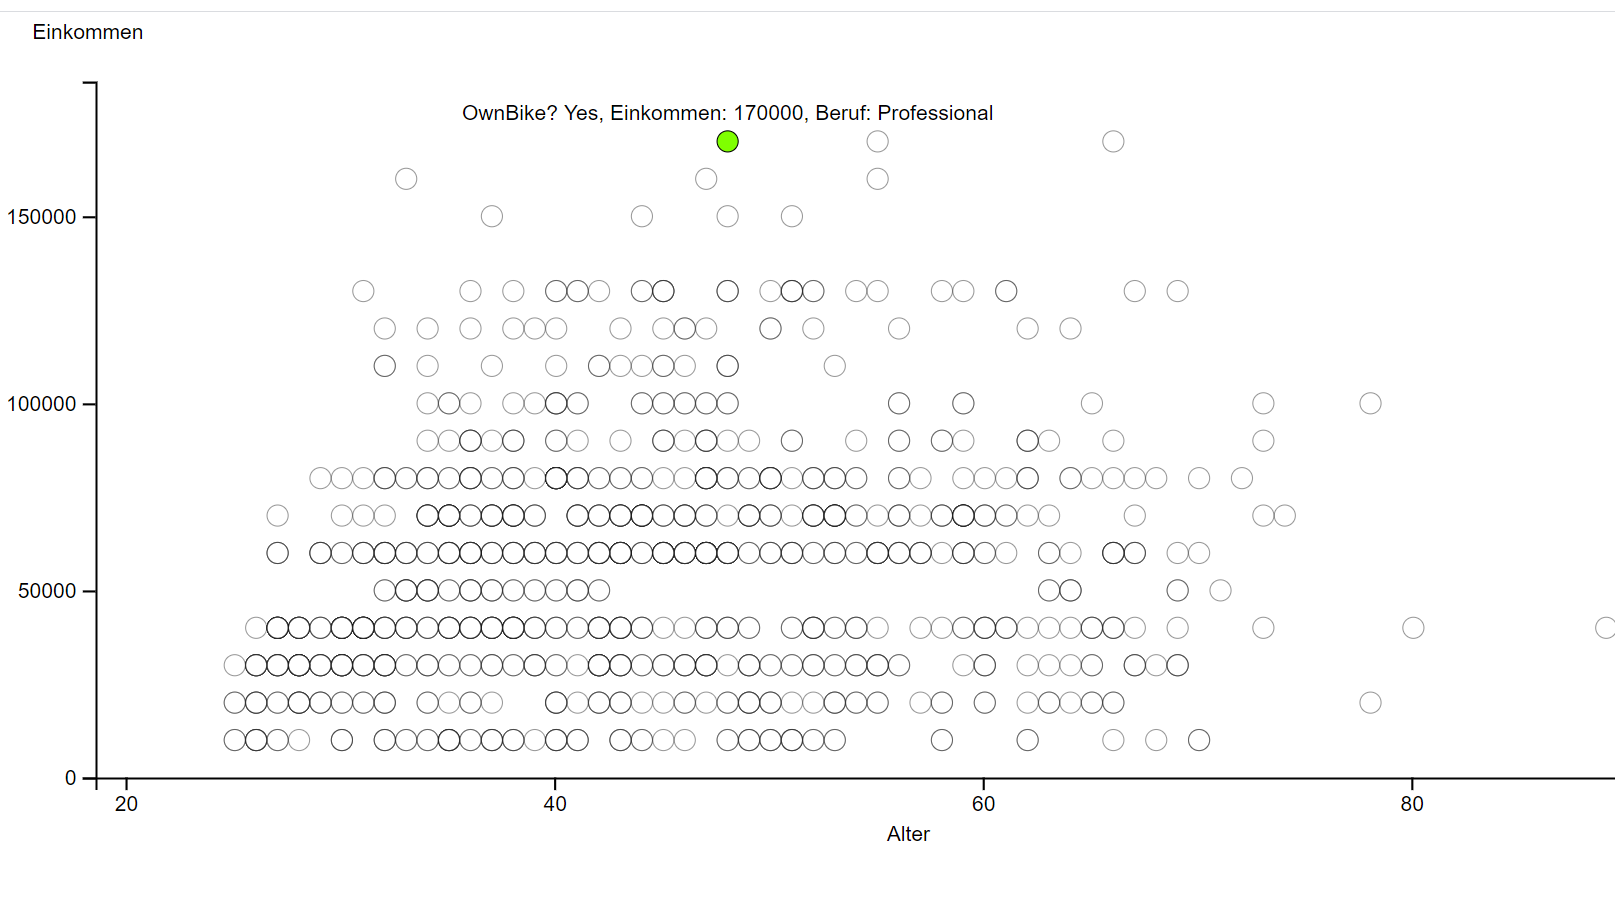
\includegraphics{Scatterplot1}

\subsubsection{Visualisierung Zwei}

TestText 123

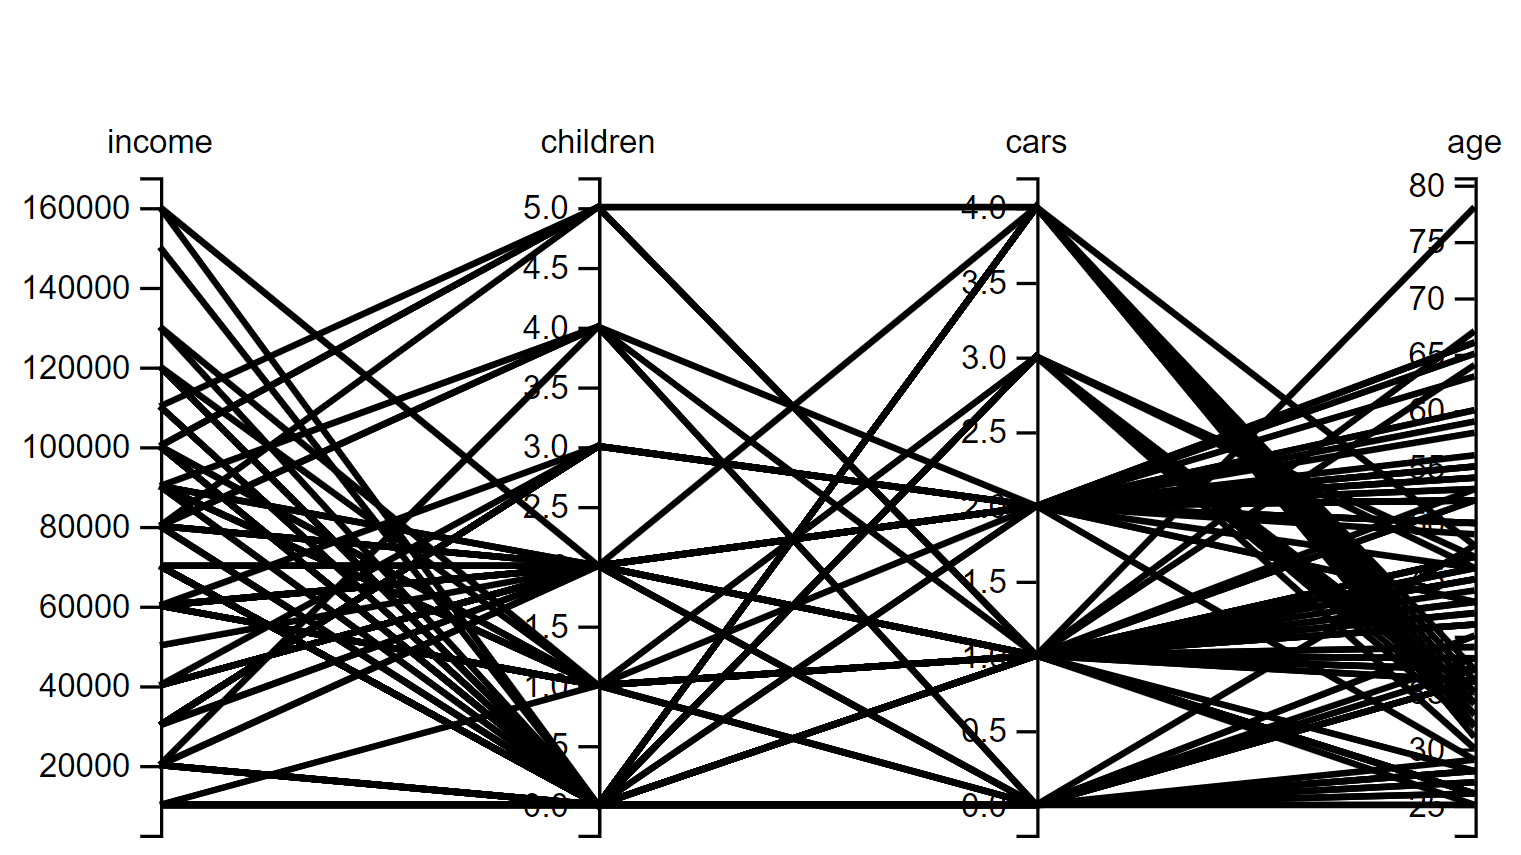
\includegraphics{parallelcoordinates}

TestText 123
\subsubsection{Visualisierung Drei}

\subsection{Interaktion}

Erklären sie die möglichen Interaktionen mit den einzelnen Visualisierungen und die möglichen Verknüpfungen zwischen ihnen. Begründen Sie warum die konkreten Interaktionen umgesetzt wurden und welche Zwecke für die Anwenderinnen mit ihnen unterstützt werden. Begründen sie ebenfalls warum sie andere Interaktionsmöglichkeiten nicht umgesetzt haben. 

\section{Implementierung}
Beschreiben Sie die Implementierung ihrer Visualisierungsanwendung in Elm. Stellen die Gliederung ihres Quellcodes vor. Haben Sie verschiedene Elm-Module erstellt. Was war aufwändig umzusetzen, was ließ sich mit dem vorhanden Code aus den Übungen relativ einfach umsetzen? 

Wie sieht die Elm-Datenstruktur für das Model aus, in dem die verschiedenen Zustände der Interaktion gespeichert werden können.

\section{Anwendungsfälle}
Präsentieren sie für jede der drei Visualisierungen einen sinnvollen Anwendungsfall in dem ein bestimmter Fakt, ein Muster oder die Abwesenheit eines Musters visuell festgestellt wird. Begründen sie warum dieser Anwendungsfall wichtig für die Zielgruppe der Anwenderinnen ist. Diskutieren sie weiterhin, ob die oben beschriebene Information auch mit anderen Visualisierungstechniken hätte gefunden werden können. Falls dies möglich wäre, vergleichen sie die den Aufwand und die Schwierigkeiten ihres Ansatzes und der Alternativen. 
\subsection{Anwendung Visualisierung Eins}
\subsection{Anwendung Visualisierung Zwei}
\subsection{Anwendung Visualisierung Drei}

\section{Verwandte Arbeiten}
Führen sie eine kurze Literatursuche in der wissenschaftlichen Literatur zu Informationsvisualisierung und Visual Analytics nach ähnlichen Anwendungen durch. Diskutieren sie mindestens zwei Artikel. Stellen sie Gemeinsamkeiten und Unterschiede dar.

\section{Zusammenfassung und Ausblick}
Fassen sie die Beiträge ihre Visualisierungsanwendung zusammen. Wo bietet sie für die Personen der Zielgruppe einen echten Mehrwert.

Was wären mögliche sinnvolle Erweiterungen, entweder auf der Ebene der Visualisierungen und/oder auf der Datenebene?

\section*{Anhang: Git-Historie}
\newpage
\bibliography{literatur}

\end{document}

